%%%%%%%%%%%%%%%%%%%%%%%%%%%%%%%%%%%%
% Section: Our Algorithm 
%%%%%%%%%%%%%%%%%%%%%%%%%%%%%%%%%%%%
\section{Our Algorithm}
\begin{frame}
\frametitle{Algorithm Overview}
\begin{itemize}
  \item Based on the simplified duplex construction with parameters:
  \begin{itemize}
    \item Width: $b = 512$
    \item Rate: $r = 128$ 
    \item Capacity: $c = 384$ 
  \end{itemize}
  \item Most design effort into pseudorandom permutation $f$
\end{itemize}
\end{frame}

\begin{frame}
\frametitle{Permutation Overview}
\begin{itemize}
  \item Permutation consists of several \emph{rounds}
  \begin{itemize}
    \item $R = 10$ for $128$-bit key
    \item $R = 16$ for $256$-bit key
  \end{itemize}
  \item Each round consists of 4 steps
  \begin{itemize}
    \item Substitution
    \item Bitwise Permutation
    \item Mixer
    \item Add Round Constant
  \end{itemize}
  \item Each step has a fairly specific purpose
\end{itemize}
\end{frame}

% TODO might be impossible to make this look good
\begin{comment}
\begin{frame}
\frametitle{Single Round Illustrated}
\begin{figure}[p]
\centering
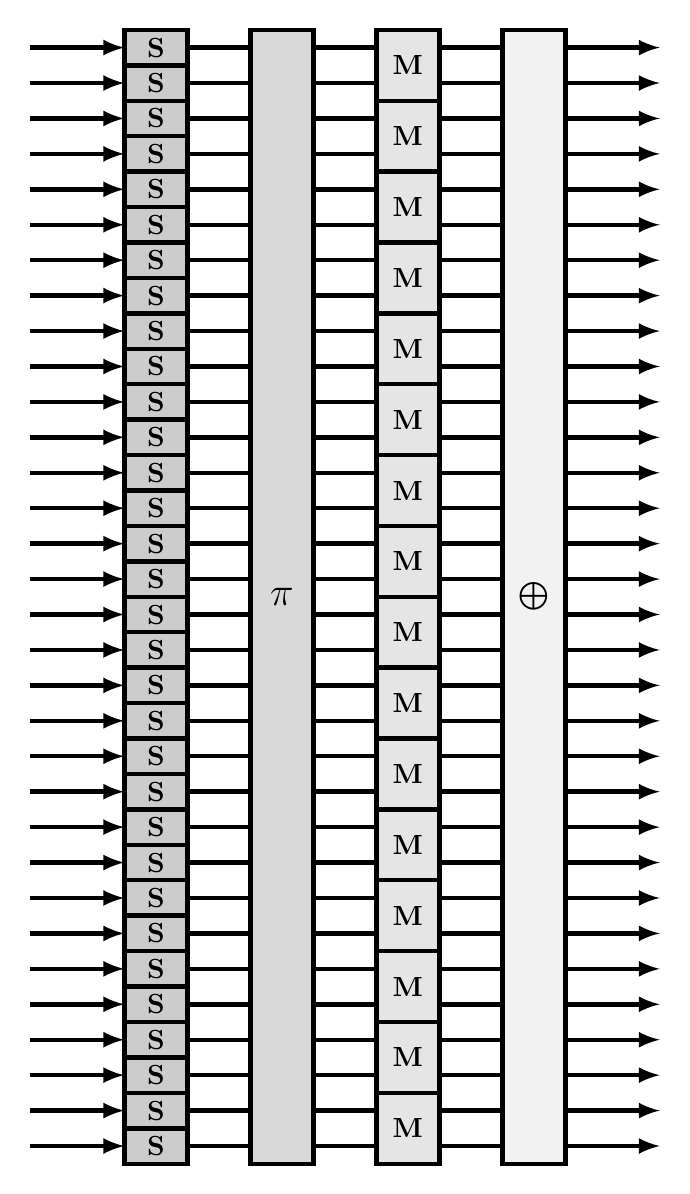
\begin{tikzpicture}[xscale=.8,yscale=0.45,>=latex,ultra thick]
% Reference grid (temporary)
%\draw[help lines] (0,0) grid (16,32);

% TODO label bits / words

% Entry arrows
\foreach \i in {32,...,1} {
  \draw[->] (-1.5,\i-0.5) -- (0,\i-0.5);
}

% Wires
\foreach \j in {1,3,5} {
  \foreach \i in {32,...,1} {
    \draw (\j,\i-0.5) -- (\j+1,\i-0.5);
  }
}

% S-boxes
\foreach \i in {32,...,1} {
  \draw[fill=gray!40] (0,\i) rectangle (1,\i-1) node[midway] {$\mathbf{S}$} ;
}

% P-boxes
\draw[fill=gray!30] (2,0) rectangle (3,32) node[midway] {\Large$\mathbf{\pi}$};

% Mixers
\foreach \i in {32,30,...,2} {
  \draw[fill=gray!20] (4,\i) rectangle (5,\i-2) node[midway] {$\mathbf{M}$};
}

% Round key box
\draw[fill=gray!10] (6,0) rectangle (7,32) node[midway] {$\bigoplus$};

% Exit arrows
\foreach \i in {32,...,1} {
  \draw[->] (7,\i-0.5) -- (8.5,\i-0.5);
}

\end{tikzpicture}


\caption{A single round of the sponge permutation $f$. Each line represents a $16$-bit word.}
\end{figure}
\end{frame}
\end{comment}

\begin{frame}
\frametitle{Single Round Illustrated}
\vfill
\begin{center}
\Large
See thesis document...sorry!
\end{center}
\vfill
\end{frame}

\begin{frame}
\frametitle{Substitution Step}
\begin{itemize}
  \item \emph{S-box}: random-looking map from $n$-bit inputs to $m$-bit outputs
  \item Main source of \emph{confusion} 
  \item We use 32 identical $16 \times 16$ S-boxes
  \item Could be randomly generated mappings with nice properties
  \begin{itemize}
    \item Not suitable for hardware
  \end{itemize}
  \item Instead based on invertible operations in a GF (similar to AES)
\end{itemize}
\end{frame}

\begin{frame}
\frametitle{S-box}
\begin{itemize}
  \item Taken from Chris Wood's MS thesis (CS Dept., 2013) \cite{Wood2013_SboxThesis}
  \item Multiplicative inversion in \gfsixteen with irreducible polynomial
  \begin{equation*}
    p(x) = x^{16} + x^5 + x^3 + x + 1
  \end{equation*} 
  \item Followed by affine transformation
  \begin{itemize}
    \item Increase algebraic complexity
  \end{itemize}
  \item Only 1238 XOR gates and 144 AND gates in hardware
\end{itemize}
\end{frame}

\begin{frame}
\frametitle{S-box Equation}
\begin{equation*}
\footnotesize
%\renewcommand{\arraystretch}{0.7} % Make it square
\begin{pmatrix}
0 & 0 & 1 & 0 & 0 & 0 & 0 & 1 & 0 & 0 & 1 & 1 & 1 & 1 & 1 & 0 \\
1 & 1 & 0 & 0 & 0 & 0 & 0 & 1 & 0 & 1 & 1 & 0 & 1 & 0 & 1 & 0 \\
1 & 1 & 0 & 0 & 1 & 0 & 1 & 1 & 0 & 1 & 0 & 1 & 0 & 0 & 1 & 1 \\
1 & 1 & 1 & 0 & 0 & 0 & 1 & 0 & 0 & 1 & 1 & 0 & 0 & 0 & 0 & 0 \\

1 & 1 & 0 & 0 & 0 & 1 & 1 & 0 & 0 & 1 & 1 & 1 & 1 & 0 & 1 & 1 \\
0 & 1 & 0 & 0 & 0 & 0 & 1 & 1 & 0 & 1 & 1 & 1 & 1 & 1 & 0 & 1 \\
0 & 0 & 1 & 0 & 1 & 0 & 1 & 0 & 1 & 1 & 0 & 0 & 1 & 1 & 0 & 0 \\
1 & 0 & 1 & 1 & 1 & 0 & 1 & 1 & 0 & 0 & 0 & 1 & 0 & 1 & 1 & 1 \\

0 & 1 & 0 & 0 & 0 & 0 & 0 & 0 & 1 & 0 & 0 & 1 & 1 & 1 & 0 & 1 \\
1 & 0 & 1 & 1 & 0 & 0 & 0 & 1 & 0 & 0 & 1 & 0 & 1 & 0 & 0 & 0 \\
1 & 0 & 1 & 0 & 0 & 1 & 1 & 1 & 0 & 0 & 1 & 1 & 0 & 1 & 0 & 0 \\
1 & 0 & 1 & 1 & 1 & 0 & 1 & 1 & 1 & 1 & 0 & 1 & 1 & 0 & 0 & 1 \\

1 & 0 & 1 & 0 & 0 & 1 & 0 & 1 & 1 & 0 & 0 & 1 & 0 & 0 & 0 & 1 \\
0 & 1 & 0 & 0 & 0 & 1 & 1 & 1 & 1 & 0 & 0 & 0 & 0 & 0 & 0 & 1 \\
1 & 0 & 0 & 0 & 1 & 1 & 0 & 1 & 0 & 1 & 1 & 1 & 1 & 0 & 0 & 0 \\
1 & 1 & 0 & 1 & 0 & 1 & 1 & 0 & 1 & 0 & 0 & 1 & 1 & 0 & 0 & 0 \\
\end{pmatrix}
\begin{pmatrix}
x_{15} \\
x_{14} \\
x_{13} \\
x_{12} \\
x_{11} \\
x_{10} \\
x_{9} \\
x_{8} \\
x_{7} \\
x_{6} \\
x_{5} \\
x_{4} \\
x_{3} \\
x_{2} \\
x_{1} \\
x_{0} \\
\end{pmatrix}
^{-1}
\oplus
\begin{pmatrix}
0 \\
1 \\
0 \\
0 \\
0 \\
1 \\
0 \\
1 \\
1 \\
0 \\
1 \\
1 \\
0 \\
1 \\
1 \\
1 \\
\end{pmatrix}
\end{equation*}
\end{frame}

\begin{frame}
\frametitle{Inverse S-box Equation}
\begin{equation*}
\footnotesize
%\renewcommand{\arraystretch}{0.7} % Make it square
\left[
\begin{pmatrix}
0 & 1 & 0 & 1 & 0 & 1 & 1 & 1 & 0 & 0 & 1 & 0 & 0 & 0 & 0 & 1 \\
1 & 1 & 0 & 1 & 0 & 0 & 1 & 0 & 1 & 0 & 1 & 1 & 1 & 1 & 0 & 1 \\
1 & 0 & 1 & 1 & 1 & 1 & 0 & 1 & 0 & 1 & 1 & 0 & 0 & 0 & 0 & 0 \\
0 & 0 & 1 & 0 & 1 & 1 & 1 & 0 & 1 & 0 & 1 & 1 & 1 & 0 & 1 & 0 \\

1 & 1 & 1 & 1 & 1 & 0 & 0 & 0 & 1 & 0 & 0 & 0 & 0 & 1 & 0 & 0 \\
0 & 0 & 0 & 1 & 0 & 1 & 0 & 0 & 0 & 0 & 1 & 1 & 1 & 1 & 1 & 1 \\
1 & 0 & 1 & 0 & 0 & 0 & 0 & 0 & 0 & 1 & 1 & 0 & 1 & 0 & 1 & 1 \\
0 & 0 & 1 & 0 & 1 & 1 & 1 & 0 & 0 & 1 & 0 & 1 & 1 & 1 & 1 & 0 \\

0 & 0 & 0 & 0 & 0 & 0 & 1 & 0 & 0 & 0 & 1 & 0 & 0 & 0 & 1 & 0 \\
1 & 1 & 1 & 0 & 0 & 1 & 1 & 1 & 1 & 0 & 1 & 1 & 1 & 0 & 0 & 0 \\
0 & 1 & 1 & 0 & 1 & 1 & 1 & 1 & 0 & 0 & 1 & 0 & 1 & 1 & 1 & 1 \\
1 & 0 & 0 & 1 & 1 & 0 & 0 & 0 & 1 & 0 & 0 & 1 & 1 & 0 & 1 & 1 \\

1 & 0 & 0 & 0 & 0 & 1 & 0 & 1 & 1 & 1 & 0 & 0 & 1 & 0 & 1 & 0 \\
1 & 0 & 0 & 0 & 0 & 1 & 1 & 1 & 1 & 1 & 0 & 1 & 1 & 1 & 1 & 1 \\
1 & 1 & 1 & 0 & 0 & 1 & 1 & 0 & 1 & 0 & 0 & 1 & 1 & 1 & 1 & 1 \\
0 & 1 & 0 & 0 & 1 & 0 & 1 & 0 & 1 & 0 & 0 & 1 & 0 & 0 & 0 & 1 \\
\end{pmatrix}
\begin{pmatrix}
x_{15} \\
x_{14} \oplus 1 \\
x_{13} \\
x_{12} \\
x_{11} \\
x_{10} \oplus 1 \\
x_{9} \\
x_{8} \oplus 1 \\
x_{7} \oplus 1 \\
x_{6} \\
x_{5} \oplus 1 \\
x_{4} \oplus 1 \\
x_{3} \\
x_{2} \oplus 1 \\
x_{1} \oplus 1 \\
x_{0} \oplus 1 \\
\end{pmatrix}
\right]^{-1}
\end{equation*}
\end{frame}

\begin{frame}
\frametitle{Bitwise Permutation}
\begin{itemize}
  \item Provides \emph{long-range diffusion}
  \item Aims to increase min number of active S-boxes
  \item Could be random mapping with nice properties
  \item We define it using an affine function with nice properties
  \item Allows for compact representation
  \begin{equation*}
  \pi(x) = 31x + 15 \pmod{512}
  \end{equation*}
  where $x \in \mathbb{Z}_{512}$ is the bit index
\end{itemize}
\end{frame}

\begin{frame}
\frametitle{Bitwise Permutation Properties}
\begin{enumerate}
  \item Sends all $16$ outputs of each S-box to 16 different mixers
  \item Has no fixed points: $\pi(x) \ne x$ for any $x$
  \item High order; does not repeat within $R$ rounds
  \item No lower order bits
\end{enumerate}
We found $384$ permutations defined by affine functions that satisfy these properties.
\end{frame}

\begin{frame}
\frametitle{PRESENT Attack}
\begin{figure}[ht]
\centering
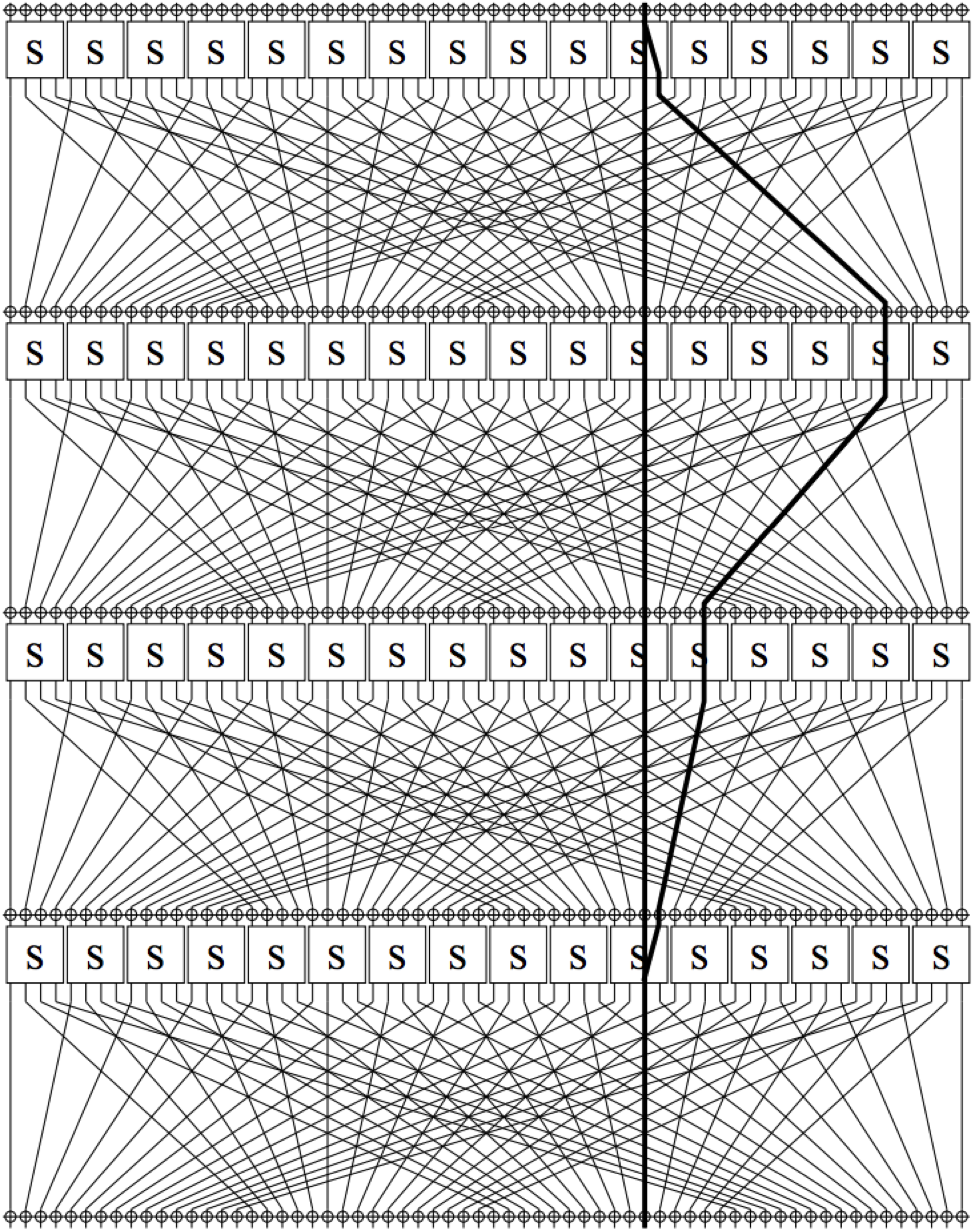
\includegraphics[height=0.62\textheight]{img/PRESENT_Trail.png}
\caption{Minimization of PRESENT active S-boxes}
\end{figure}
\end{frame}

\begin{frame}
\frametitle{Mixer}
\begin{itemize}
  \item Increase \emph{branch number} of round to 3
  \begin{itemize}
    \item Verified via SAT solver analysis 
    \item Tools courtesy of Alan Kaminsky
  \end{itemize}
  \item Provide local diffusion
  \item Defined by invertible matrix multiplication in \gfsixteen
  \item Irreducible polynomial:
  \begin{equation*}
  p(x) = x^{16} + x^5 + x^3 + x^2 + 1
  \end{equation*}
\end{itemize}
\end{frame}

\begin{frame}
\frametitle{Mixer Equations}
\begin{itemize}
  \item Input two words $A$ and $B$
  \item Forward:
  \begin{equation*}
  \begin{pmatrix}
  A' \\ B'
  \end{pmatrix}
  =
  \begin{pmatrix}
  1 & x \\ x & x + 1
  \end{pmatrix}
  \begin{pmatrix}
  A \\ B
  \end{pmatrix}
  \end{equation*}
  
  \item Inverse: 

\begin{equation*}
\begin{pmatrix}
A \\ B
\end{pmatrix}
=
\begin{pmatrix}
a & b \\ b & c
\end{pmatrix}
\begin{pmatrix}
A' \\ B'
\end{pmatrix}
\end{equation*}
where
\begin{align*}
a &= x^{15} + x^{14} + x^{12} + x^{11} + x^9 + x^8 + x^6 + x^5 + x^4 + x + 1 \\
b &= x^{14} + x^{13} + x^{11} + x^{10} + x^8 + x^7 + x^5 + x^4 + x^3 + 1 \\
c &= x^{15} + x^{13} + x^{12} + x^{10} + x^9 + x^7 + x^6 + x^3 + x.
\end{align*}
\end{itemize}
\end{frame}

\begin{frame}
\frametitle{Mixer in Hardware}
\begin{figure}[ht]
\centering
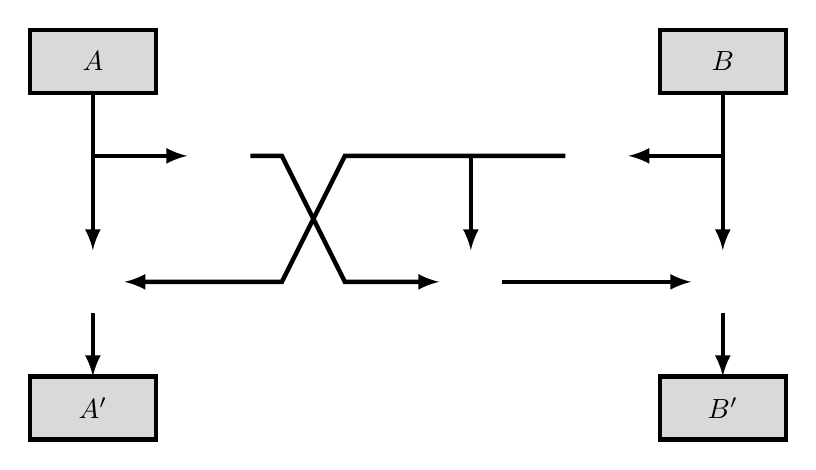
\begin{tikzpicture}[xscale=0.8,yscale=0.8,>=latex,ultra thick]
% Reference grid (temporary)
%\draw[help lines] (0,0) grid (16,16);

% Inputs
\draw[fill=gray!30] (0,15) rectangle (2,14) node[midway] {$A$};
\draw[fill=gray!30] (10,15) rectangle (12,14) node[midway] {$B$};

\draw[->] (1,14) to (1, 11.5);
\draw[->] (1,13) to (2.5, 13);

\draw[->] (11,14) to (11, 11.5);
\draw[->] (11,13) to (9.5, 13); 

\drawxTimes{3}{13}
\drawxTimes{9}{13}

\drawXOR{1}{11}
\drawXOR{11}{11}
\drawXOR{7}{11}

\draw[->] (3.5,13) to (4,13) to (5,11) to (6.5,11);
\draw[->] (8.5,13) to (5,13) to (4,11) to (1.5,11); 
\draw[->] (7,13) to (7,11.5);
\draw[->] (7.5,11) to (10.5,11);

\draw[->] (1,10.5) to (1,9.5);
\draw[->] (11,10.5) to (11,9.5);

% Outputs
\draw[fill=gray!30] (0,9.5) rectangle (2,8.5) node[midway] {$A'$};
\draw[fill=gray!30] (10,9.5) rectangle (12,8.5) node[midway] {$B'$};

\end{tikzpicture}

\caption{Hardware implementation of forward mixer function.}
\end{figure}
\end{frame}

\begin{frame}
\frametitle{$x*$ in Hardware}
\begin{figure}[ht]
\centering
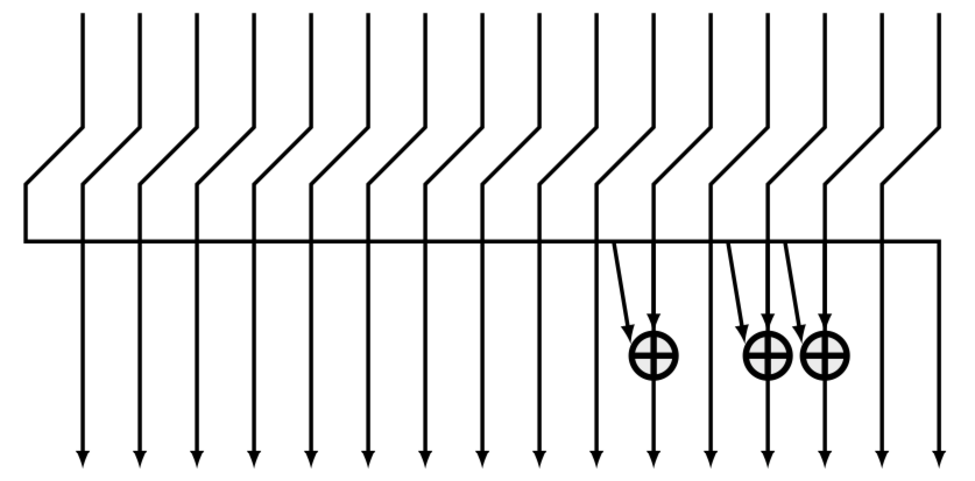
\includegraphics[width=\textwidth]{img/xTimes.pdf}
\caption{Hardware implementation of the $x*$ function. The leftmost bit is the MSB.}
\end{figure}
\end{frame}

\begin{frame}
\frametitle{Add Round Constant}
\begin{itemize}
  \item Very simple; its own inverse
  \item Bitwise XOR $512$-bit round constant into state
  \item Reduces symmetry in state
  \item Prevents against \emph{slide attacks}
  \item RCs generated as follows:
  \begin{equation*}
  RC_i = \mathbf{SHA3\textbf{-}512}(\mathbf{ASCII}(i))
  \end{equation*}
\end{itemize}
\end{frame}

\begin{frame}
\frametitle{Customization}
\begin{itemize}
  \item Different S-box from Wood's thesis
  \begin{itemize}
    \item Recalculate maximum linear bias and differential probabilities
  \end{itemize}
  \item Different bitwise permutation out of the $384$ we found
  \item Different matrix for mixer
  \begin{itemize}
    \item Verify branch number is 3 using SAT tools 
  \end{itemize} 
  \item Different round constants
\end{itemize}
\end{frame}

